%----------------------------------------------------------------------------------------
%	THE OSCILLATOR.
%----------------------------------------------------------------------------------------
\subsection{The oscillator}


\begin{figure}[H]
\centering
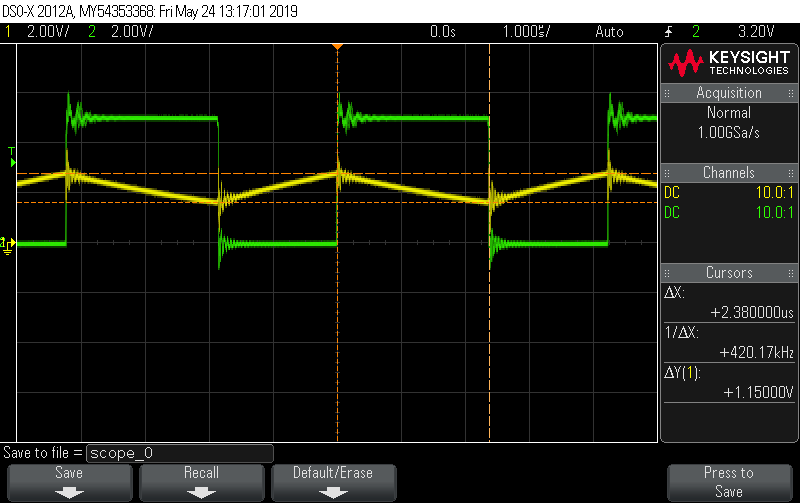
\includegraphics[width=.9\textwidth]{figures/scope_0.png}
\caption{The Schmitt trigger circuit (oscillator) with yellow being the input 'TCP' and green the output 'OSC-OP' at a random frequency.}
\label{fig:scope_0}
\end{figure}


\begin{figure}[H]
\centering
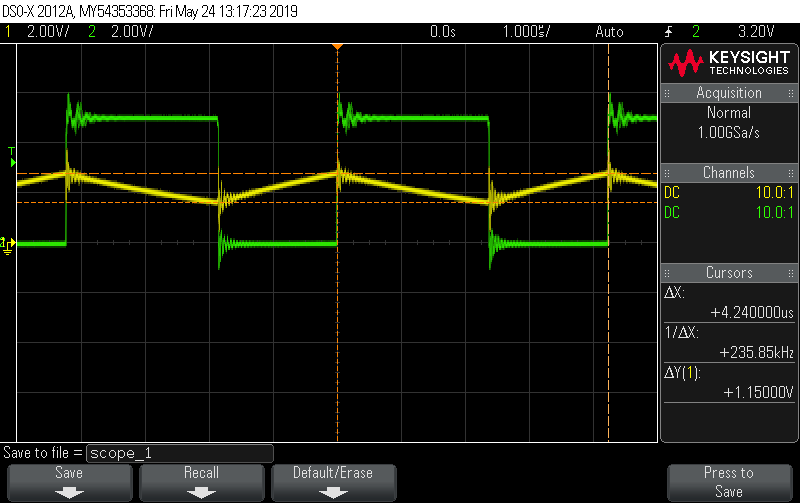
\includegraphics[width=.9\textwidth]{figures/scope_1.png}
\caption{The Schmitt trigger circuit (oscillator) with yellow being the input 'TCP' and green the output 'OSC-OP' at a random frequency.}
\label{fig:scope_1}
\end{figure}


\begin{figure}[H]
\centering
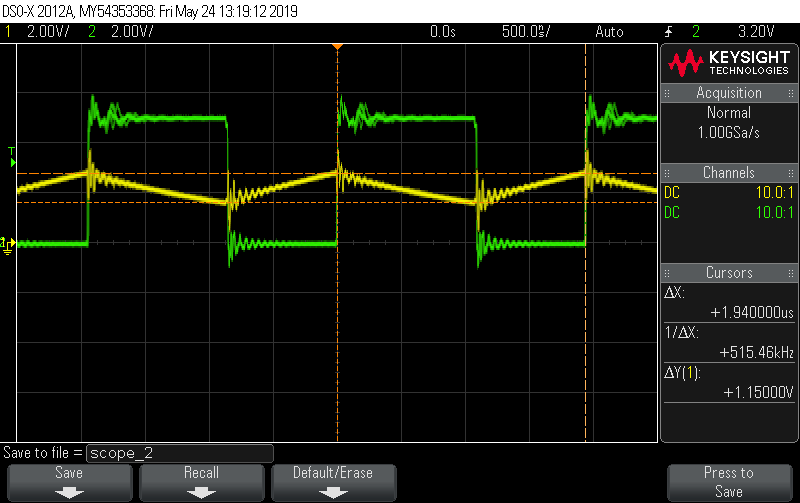
\includegraphics[width=.9\textwidth]{figures/scope_2.png}
\caption{The Schmitt trigger circuit (oscillator) with yellow being the input 'TCP' and green the output 'OSC-OP' with the maximum frequency.}
\label{fig:scope_2}
\end{figure}


\begin{figure}[H]
\centering
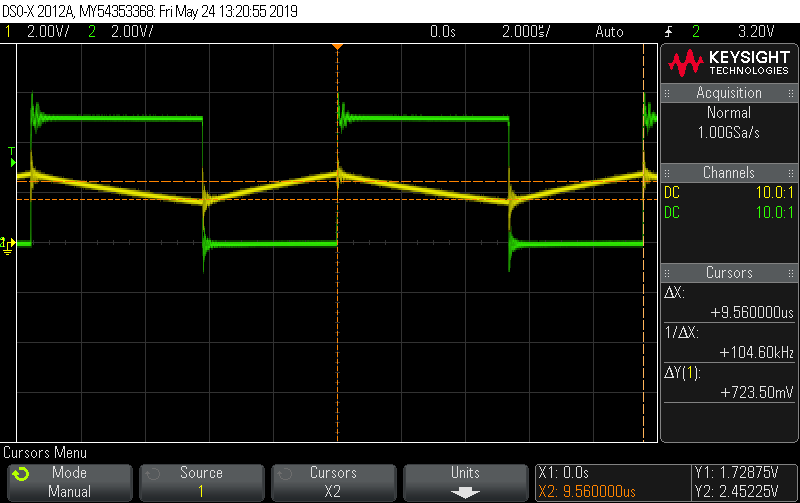
\includegraphics[width=.9\textwidth]{figures/scope_3.png}
\caption{The Schmitt trigger circuit (oscillator) with yellow being the input 'TCP' and green the output 'OSC-OP' with the minimum frequency.}
\label{fig:scope_3}
\end{figure}

